\documentclass[11pt]{article}
\usepackage{microtype}
\usepackage{graphicx}
\usepackage{wrapfig}
\usepackage{url}
\usepackage{wrapfig}
\usepackage{color}
\usepackage{marvosym}
\usepackage{enumerate}
\usepackage{subfigure}
\usepackage{tikz}
\usepackage[fleqn]{amsmath}
\DeclareMathOperator*{\argmax}{arg\,max}
\DeclareMathOperator*{\argmin}{arg\,min}
\usepackage{amssymb}
\usepackage{hyperref}
\usepackage[many]{tcolorbox}
\usepackage{lipsum}
\usepackage{float}
\usepackage{trimclip}
\usepackage{listings}
\usepackage{environ}% http://ctan.org/pkg/environ
\usepackage{wasysym}
\usepackage{array}
\usepackage{booktabs}


\oddsidemargin 0mm
\evensidemargin 5mm
\topmargin -20mm
\textheight 240mm
\textwidth 160mm

\newcommand{\vwi}{{\bf w}_i}
\newcommand{\vw}{{\bf w}}
\newcommand{\vx}{{\bf x}}
\newcommand{\vy}{{\bf y}}
\newcommand{\vxi}{{\bf x}_i}
\newcommand{\yi}{y_i}
\newcommand{\vxj}{{\bf x}_j}
\newcommand{\vxn}{{\bf x}_n}
\newcommand{\yj}{y_j}
\newcommand{\ai}{\alpha_i}
\newcommand{\aj}{\alpha_j}
\newcommand{\X}{{\bf X}}
\newcommand{\Y}{{\bf Y}}
\newcommand{\vz}{{\bf z}}
\newcommand{\msigma}{{\bf \Sigma}}
\newcommand{\vmu}{{\bf \mu}}
\newcommand{\vmuk}{{\bf \mu}_k}
\newcommand{\msigmak}{{\bf \Sigma}_k}
\newcommand{\vmuj}{{\bf \mu}_j}
\newcommand{\msigmaj}{{\bf \Sigma}_j}
\newcommand{\pij}{\pi_j}
\newcommand{\pik}{\pi_k}
\newcommand{\D}{\mathcal{D}}
\newcommand{\el}{\mathcal{L}}
\newcommand{\N}{\mathcal{N}}
\newcommand{\vxij}{{\bf x}_{ij}}
\newcommand{\vt}{{\bf t}}
\newcommand{\yh}{\hat{y}}
\newcommand{\code}[1]{{\footnotesize \tt #1}}
\newcommand{\alphai}{\alpha_i}
\newcommand{\defeq}{\overset{\text{def}}{=}}
\renewcommand{\vec}[1]{\mathbf{#1}}



\bgroup
\def\arraystretch{1.5}
\newcolumntype{x}[1]{>{\centering\arraybackslash\hspace{0pt}}p{#1}}
\newcolumntype{z}[1]{>{\centering\arraybackslash}m{#1}}

%Arguments are 1 - height, 2 - box title
\newtcolorbox{textanswerbox}[2]{%
 width=\textwidth,colback=white,colframe=blue!30!black,floatplacement=H,height=#1,title=#2,clip lower=true,before upper={\parindent0em}}

 \newtcolorbox{eqanswerbox}[1]{%
 width=#1,colback=white,colframe=black,floatplacement=H,height=3em,sharp corners=all,clip lower=true,before upper={\parindent0em}}

 %Arguments are 1 - height, 2 - box title
 \NewEnviron{answertext}[2]{
        \noindent
        \marginbox*{0pt 10pt}{
        \clipbox{0pt 0pt 0pt 0pt}{
        \begin{textanswerbox}{#1}{#2}
        \BODY
        \end{textanswerbox}
        }
        }
}

%Arguments are 1 - height, 2 - box title, 3 - column definition
 \NewEnviron{answertable}[3]{
        \noindent
        \marginbox*{0pt 10pt}{
        \clipbox{0pt 0pt 0pt 0pt}{
        \begin{textanswerbox}{#1}{#2}
                \vspace{-0.5cm}
                        \begin{table}[H]
                        \centering
                        \begin{tabular}{#3}
                                \BODY
                        \end{tabular}
                        \end{table}
        \end{textanswerbox}
        }
        }
}

 %Arguments are 1 - height, 2 - box title, 3 - title, 4- equation label, 5 - equation box width
 \NewEnviron{answerequation}[5]{
        \noindent
        \marginbox*{0pt 10pt}{
        \clipbox{0pt 0pt 0pt 0pt}{
        \begin{textanswerbox}{#1}{#2}
                \vspace{-0.5cm}
                        \begin{table}[H]
                        \centering
                \renewcommand{\arraystretch}{0.5}% Tighter

                        \begin{tabular}{#3}
                                #4 =	&
                        \clipbox{0pt 0pt 0pt 0pt}{

                        \begin{eqanswerbox}{#5}
                                $\BODY$
                        \end{eqanswerbox}
                        } \\
                        \end{tabular}
                        \end{table}

        \end{textanswerbox}
        }
        }
}

 %Arguments are 1 - height, 2 - box title
 \NewEnviron{answerderivation}[2]{
        \noindent
        \marginbox*{0pt 10pt}{
        \clipbox{0pt 0pt 0pt 0pt}{
        \begin{textanswerbox}{#1}{#2}
        \BODY
        \end{textanswerbox}
        }
        }
}

\newcommand{\Checked}{{\LARGE \XBox}}%
\newcommand{\Unchecked}{{\LARGE \Square}}%
\newcommand{\TextRequired}{{\textbf{Place Answer Here}}}%
\newcommand{\EquationRequired}{\textbf{Type Equation Here}}%


\newcommand{\answertextheight}{5cm}
\newcommand{\answertableheight}{4cm}
\newcommand{\answerequationheight}{2.5cm}
\newcommand{\answerderivationheight}{14cm}

\newcounter{QuestionCounter}
\newcounter{SubQuestionCounter}[QuestionCounter]
\setcounter{SubQuestionCounter}{1}

\newcommand{\subquestiontitle}{Question \theQuestionCounter.\theSubQuestionCounter~}
\newcommand{\newquestion}{\stepcounter{QuestionCounter}\setcounter{SubQuestionCounter}{1}\newpage}
\newcommand{\newsubquestion}{\stepcounter{SubQuestionCounter}}


\lstset{language=[LaTeX]TeX,basicstyle=\ttfamily\bf}

\pagestyle{myheadings}
\markboth{Homework 5}{Fall 2020 CS 475/675 Machine Learning: Homework 5 Analytical}

\title{CS 475 Machine Learning: Homework 5\\
Deep Learning: Analytical\\
\Large{Due: Thursday November 12, 11:59pm}\\
40 Points Total \hspace{1cm} Version 1.0}
\author{PARTNER1\_NAME (PARTNER1\_JHED), PARTER2\_NAME (PARTNER2\_JHED)}
\date{}

\begin{document}
\maketitle
\thispagestyle{headings}

\section*{Homework 5}
For the remaining homeworks, we will combine all three homework types into single assignments. Both homework 5 and 6 will be worth 100 points. Homeworks 1-6 will be worth a total of 400.

Homework 5 has three parts totalling 100 points. 
\begin{enumerate}
    \item Analytical (40 points)
    \item Programming (45 points)
    \item Lab (15 points)
\end{enumerate}

All three parts of the homework have the same due date. Late hours will be counted based on when the last part is submitted. 

For this assignment you may only work with a partner on the analytical section.

\section*{Instructions }
We have provided this \LaTeX{} document for turning in this homework. We give you one or more boxes to answer each question.  The question to answer for each box will be noted in the title of the box.\\

{\bf Other than your name, do not type anything outside the boxes. Leave the rest of the document unchanged.}\\


\textbf{Do not change any formatting in this document, or we may be unable to
  grade your work. This includes, but is not limited to, the height of
  textboxes, font sizes, and the spacing of text and tables.  Additionally, do
  not add text outside of the answer boxes. Entering your answers are the only
  changes allowed.}\\


\textbf{We strongly recommend you review your answers in the generated PDF to
  ensure they appear correct. We will grade what appears in the answer boxes in
  the submitted PDF, NOT the original latex file.}

\pagebreak

\section*{ Notation}
{
\centering
\smallskip\begin{tabular}{r l}
\(\vec{x_i}\) & One input data vector. \(\vec{x_i}\) is \(M\) dimensional.
\(\vec{x_i} \in \mathbb{R}^{1 \times M}\).  \\ &
We assume $\vec{x_i}$ is augmented with a  $1$ to include a bias term. \\ \\
\(\vec{X}\) & 	A matrix of concatenated \(\vec{x_i}\)'s. There are \(N\) input vectors, so \(\vec{X} \in \mathbb{R}^{N \times M}\) \\ \\
\(y_i\) & The true label for input vector \(\vec{x_i}\). In regression problems, \(y_i\) is continuous. \\ & In general ,\(y_i\) can be a vector, but for now we assume it's a scalar: \(y_i \in \mathbb{R}^1\). \\ \\

\(\vec{y}\) & 	A vector of concatenated \(y_i\)'s. There are \(N\) input vectors, so \(\vec{y} \in \mathbb{R}^{N \times 1}\) \\ \\

\(\vec{w}\) & A weight vector. We are trying to learn the elements of \(\vec{w}\). \\
& \(\vec{w}\) is the same number of elements as \(\vec{x_i}\) because we will end up computing \\
& the dot product \(\vec{x_i} \cdot \vec{w}\). \\
& \(\vec{w} \in \mathbb{R}^{M \times 1}\). We assume the bias term is included in \(\vec{w}\). \\ \\

\(h(\vec(x))\) & The true regression function that describes the data. \\ \\
 
i.i.d. & Independently and identically distributed. \\ \\

Bias-variance  & We can write \(E_D[(f(x, D) - h(x))^2]\) = \\
decomposition  & \((E_D[f(x, D) - h(x))^2 + E_D[(f(x, D) - E_D[f(x, D)])^2]\) \\
                            & where the first term is the bias squared, and the second term is the variance.\\ \\

 Notes: & In general, a lowercase letter (not boldface), $a$, indicates a scalar. \\
  & A boldface lowercase letter, $\vec{a}$, indicates a vector. \\  &  A boldface uppercase letter, $\vec{A}$, indicates a matrix. \\
\end{tabular}
}
%%%%%%%%%%%%%%%%%%%%%%%%%%%%%%%%%%%%%%%%%%%%%%%%%%%%%%%%%%%%%%%%%%%%%%%%%%%%%%%%
\newquestion
\section*{\arabic{QuestionCounter}) Neural Network Construction (15 points)}

MNIST is a popular dataset of images of hand-written digits. There are 10 digits (0 through 9) to classify. Each image in the dataset is 28x28 pixels, and the images are 1-channel grayscale images. Because of the simplicity of this dataset, it is possible to achieve good results by flattening images into 1-dimensional vectors and then training a multi-layer perceptron (MLP). Suppose we have a MLP with two hidden, fully connected layers:

\begin{center}
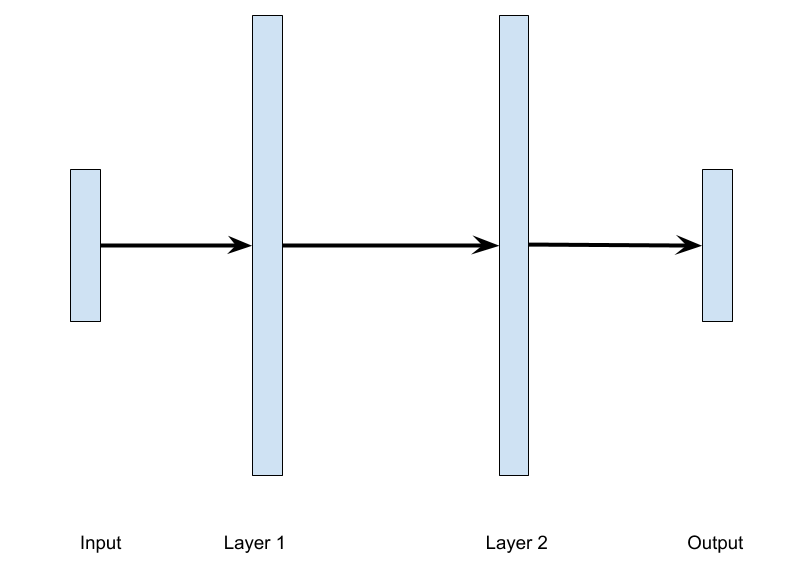
\includegraphics[width = 0.5\textwidth]{nn.png}
\end{center}

Here, the input image is flattened into a 1-dimensional vector, and y is a multi-class categorical output with a probability assigned to each of the 10 digit classes (i.e. from a softmax activation). Assume each hidden layer has 100 neurons and denote the softmax activation functions as $\sigma$. The ReLU activation function is applied after Layer 1.

\begin{enumerate}[{(a)}]

\item (5 points) Assuming there are no bias terms, express the forward pass of an image through this MLP. Denote the weights of layers 1 and 2 as $W_1$ and $W_2$, respectively. Let X denote the vector of inputs. You can express the forward pass using multiplication of matrices. 


\begin{answertext}{9cm}{}
\end{answertext} 

\item (5 points) How many parameters are there in each layer of the network? 


\begin{answertext}{9cm}{}
  
\end{answertext} 

\item (5 points) Suppose we switch to a different dataset where the images are provided as high quality images (2000 x 2000 pixels) and images are now in color, where each pixel is represented by a RBG value (a triplet of integers between 0 and 255). Do you think the MLP used in the previous parts of the question will do well on this dataset? Why or why not?

\begin{answertext}{10cm}{}
    
  
  
\end{answertext} 

\end{enumerate}

\newpage
\newquestion
\section*{\arabic{QuestionCounter}) D-Separation (10 points)}

The given diagram represents a Bayesian Network or DAG over random variables $X, Y, Z, W, U$

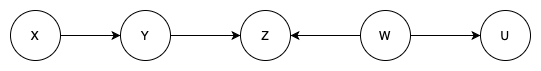
\includegraphics[scale = 0.75]{dsep.png}

Using the properties of d-separation, which of the following independence statements are true in the DAG above?
Give a one sentence explanation for each answer. The notation $X \perp Z | Y$ means that $X$ is independent of $Z$ given $Y$.

\begin{enumerate}[(a)]
    \item $X \perp Z$
    \item $Z \perp U$
    \item $X \perp U$
    \item $X \perp U \mid Z$
    \item $Z \perp U \mid W$
    \item $X \perp Z \mid Y$
    \item $X \perp W \mid \{Y, Z\}$
\end{enumerate}

\begin{answertext}{6cm}{}
    
  \begin{enumerate}[(a)]
    \item 
    \item 
    \item 
    \item 
    \item 
    \item 
    \item 
\end{enumerate}
\end{answertext} 

%%%%%%%%%%%%%%%%%%%%%%%%%%%%%%%%%%%%%%%%%%%%%%%%%%%%%%%%%%%%%%%%%%%%%%%%%%%%%%%%
\newquestion
\section*{\arabic{QuestionCounter}) Backpropagation (15 points)}

Suppose you have the following function \begin{align*}
    p &= \sigma(h_1 \cdot \sigma(w_1 x_1 + w_2 x_2) + h_2 \cdot \sigma(w_3 x_1 + w_4 x_2))\\
    L(p, y) &= - y \log{p} - (1 - y) \log(1 - p)
\end{align*}

Here $\sigma$ denotes the sigmoid activation function and $y$ is a binary label.
Consider this computation graph that represents the above computation

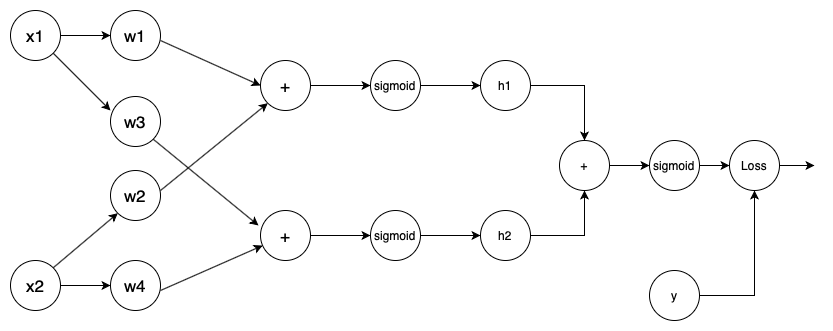
\includegraphics[width = 0.75\textwidth]{backprop-Page-1-2.png}

We will use backpropagation to compute the gradients of the loss with respect to $w_1, w_2, w_3, w_4, h_1, h_2$.


To demonstrate, let's compute $\frac{\partial L}{\partial h_1}$. To simplify notation, we will denote terms as follows
\begin{align*}
    z &= h_1 \cdot \sigma(w_1 x_2 + w_2 x_2) + h_2\cdot\sigma(w_3 x_1 + w_4 x_2)\\
    l_{12} &= w_1 \cdot x_2 + w_2 \cdot x_2\\
    l_{34} &= w_3 \cdot x_1 + w_2 \cdot x_2
\end{align*}


Using the chain rule, this can be written as $\frac{\partial L}{\partial h_1}$

\begin{align*}
    \frac{\partial L}{\partial h_1} = \frac{\partial L}{\partial p} \cdot \frac{\partial p}{\partial z} \cdot \frac{\partial z}{\partial h_1}
\end{align*}

And so, $\frac{\partial L}{\partial h_1}$ can be written as the product of gradients computed at individual nodes in the computational graph.
\newpage
\begin{enumerate}[(a)]

\item (4 Points)
Write out the expressions for the following derivatives.
\vspace{-2em}
{
\setlength{\tabcolsep}{1em}
\setlength{\extrarowheight}{1em}%
\begin{center}
\begin{tabular}{l l}
(i)  $\dfrac{\partial}{\partial q} -z \log{q} - (1 - z) \log(1 - q) $ &
(ii) $\dfrac{\partial}{\partial g_1} (g_1*a_1 + g_2*a_2)$ \\
(iii)$\dfrac{\partial}{\partial z}\sigma(z)$ &
(iv) $\dfrac{\partial}{\partial g_1} (g_1 + g_2)$ \\
\end{tabular}
\end{center}
}

\begin{answertext}{12cm}{}
% be sure to label your answers (i) to (iv)
  
\end{answertext} 
\newpage 
\item (4 points) Using the chain rule of calculus, write out the following expressions in terms of
the partial derivatives, but do not evaluate the actual backpropagation updates.
\vspace{-2em}
{
\setlength{\tabcolsep}{1em}
\setlength{\extrarowheight}{1em}%
\begin{center}
\begin{tabular}{c c c}
(i)  $\dfrac{\partial}{\partial h_1} L$ &
(ii) $\dfrac{\partial}{\partial h_2} L$ &
(iii)$\dfrac{\partial}{\partial w_1} L$ \\
(iv) $\dfrac{\partial}{\partial w_2} L$ & 
(v)  $\dfrac{\partial}{\partial w_3} L$ & 
(vi) $\dfrac{\partial}{\partial w_4} L$ \\
\end{tabular}
\end{center}
}

\begin{answertext}{12cm}{}
    
  
\end{answertext} 

\clearpage

\item (4 points)
Using the backpropagation algorithm and your answers from part (a) and (b), evaluate the value of the partial derivatives in (b) at $x_1 = 1, x_2 = -1, y = 1, w_1 = 3, w_2 = 2, w_3 = -1, w_4 = 5, h_1 = 2.5, h_2 = 1.5 $.

\begin{answertext}{8cm}{}
    
  
\end{answertext} 
\item (3 points) Instead of sigmoid activation, assume the intermediate layers use ReLU activations. How do the values of the gradients change? 

\begin{answertext}{8cm}{}
    
  
\end{answertext} 

\end{enumerate}

\end{document}
